%-----------------------------------LICENSE------------------------------------%
%   This file is part of tikz_figures.                                         %
%                                                                              %
%   tikz_figures is free software: you can redistribute it and/or              %
%   modify it it under the terms of the GNU General Public License as          %
%   published by the Free Software Foundation, either version 3 of the         %
%   License, or (at your option) any later version.                            %
%                                                                              %
%   tikz_figures is distributed in the hope that it will be useful,            %
%   but WITHOUT ANY WARRANTY; without even the implied warranty of             %
%   MERCHANTABILITY or FITNESS FOR A PARTICULAR PURPOSE.  See the              %
%   GNU General Public License for more details.                               %
%                                                                              %
%   You should have received a copy of the GNU General Public License along    %
%   with tikz_figures.  If not, see <https://www.gnu.org/licenses/>.           %
%------------------------------------------------------------------------------%

% Use the standalone class for displaying the tikz image on a small PDF.
\documentclass[crop, tikz]{standalone}

% Import the tikz package to use for the drawing.
\usepackage{tikz}

% tikz packages used.
\usetikzlibrary{arrows.meta}

% Begin the document.
\begin{document}

    % Begin the drawing.
    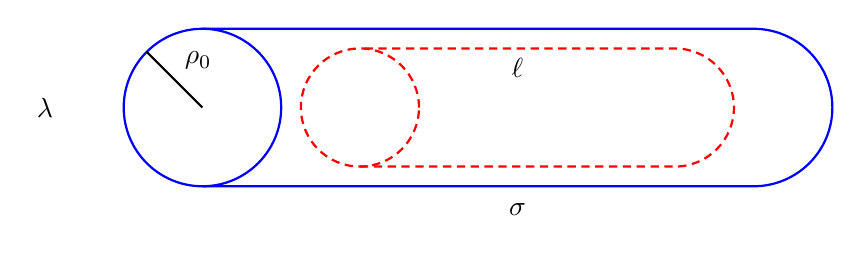
\begin{tikzpicture}[every path/.style = thick]

        % Coordindates for all of the points.
        \coordinate (A0) at (-6.0, 0.0);
        \coordinate (A1) at (-6.0, 0.0);
        \coordinate (B0) at (-4.0, 0.0);
        \coordinate (C0) at (-4.0, 1.0);
        \coordinate (C1) at (3.0, 1.0);
        \coordinate (C2) at (-4.0, -1.0);
        \coordinate (D0) at (-2.0, 0.0);
        \coordinate (E0) at (-2.0, -0.75);
        \coordinate (E1) at (2.0, -0.75);
        \coordinate (E2) at (-2.0, 0.75);
        \coordinate (F0) at (-4.0, 0.0);
        \coordinate (F1) at (-4.71, 0.71);
        \draw (A0) to (A1);

        % THe outer cylinder.
        \begin{scope}[%
            draw = blue
        ]
            \draw (B0) circle (1);
            \draw (C0) to (C1) arc (90:-90:1) to (C2);
        \end{scope}

        % The inner cylinder.
        \begin{scope}[%
            draw = red,
            densely dashed
        ]
            \draw (D0) circle (0.75);
            \draw (E0) to (E1) arc (-90:90:0.75) to (E2);
        \end{scope}

        % Straight line indicating the radial part of the cylinder.
        \draw (F0) to node[above right] {$\rho_{0}$} (F1);

        % Label everything.
        \node at (0.0, 0.5) {$\ell$};
        \node at (0.0, -1.3) {$\sigma$};
        \node at (-6.0, 0.0) {$\lambda$};
    \end{tikzpicture}
\end{document}
